\documentclass[a4paper]{article}
% Eso define el tipo de documento.
% `article` se divide en secciones y tiene el resumen pegado al texto
\usepackage{graphicx}
% Son como los import de librerias. `graphicx` es para importar imagenes
\usepackage{listings}
% `listings` es para insertar los codigo fuente
\usepackage[utf8]{inputenc}
% `utf8` es para no tener problemas con el encoding (acentos, etc.)
\usepackage{nameref}
% Para referenciar por título y no por numero con \nameref
\usepackage{untref}
% Nuestra configuracion

\title{Trabajo Práctico Nro. 2:\\“Puertos Analógicos”}
\author{Amodey, Leandro - leandroamodey@gmail.com
\and Monti, Matías - matiasmonti@hotmail.com
\and Quinteros, Fernando - lordfers@gmail.com
\and Araneda, Alejandro – eloscurodeefeso@hotmail.com}
\date{1er. Cuatrimestre 2020\\Lunes, 11 de Mayo, 8hs.}
% `title`, `author` y `date` es informacion que todos los archivos tienen.

\teacher{Ing. Jorge H. Doorn
\and Ing. Matías Presso}
% Comando propio para definir profesores.

\begin{document}
% Arranca el documento

\maketitle % Pone la caratula

\begin{abstract}

    En el presente trabajo ejemplificaremos mediante diversar 
    aplicaciones la utilización de los módulos analógicos de un 
    microcontrolador. A su vez, éstas ilustrarán la forma en que el 
    diseño digital que en general pertenece al dominio de la 
    corriente contínua y de baja tensión, se relaciona con los 
    componentes electrónicos propios también de la corriente alterna 
    y de mayor tensión.

\end{abstract}

\section{Introducción}\label{sec:teoria}
Dummy text

\subsection*{Tecnologías CMOS y TTL}
% Fijarse que este tiene * para que no se numere.

Por tecnología TTL (en inglés, \textit{transistor-transistor logic})
nos referimos a aquella que utiliza transistores de unión bipolar o 
BJT (en inglés, \textit{bipolar junction transistor}), para la 
construcción de circuitos digitales\cite{bib:boylestad}.

En cambio, los CMOS (en inglés, \textit{complementary 
metal-oxide-semiconduc-tor}) son un tipo de implementación de 
transistores de efecto de campo de la familia de los MOSFET (en 
inglés, \textit{metal-oxide-semiconductor field-effect transistor}). 
La denominación se ha mantenido a pesar de haberse generalizado el 
uso de silicio en vez de metal y otros aislantes en reemplazo del 
óxido.

\begin{figure}[h]
    \centering
    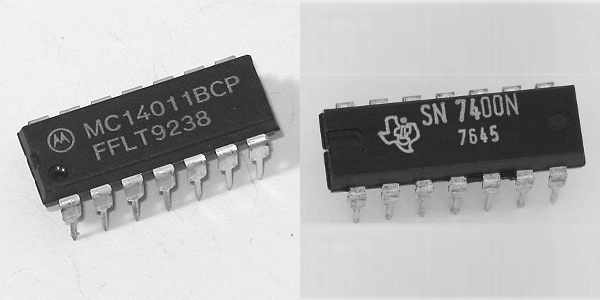
\includegraphics[height=4cm]{transistores.png}
    \caption{Integrados con tecnologías CMOS (izquierda) y TTL 
    (derecha)}
    \label{fig:transistores}
\end{figure}
% 

Las diferencias entre los transistores de tecnología BJT y los de 
tecnología FET, vienen dadas por la forma en la que cada tipo de 
componente controla el paso de corriente de la terminal colectora a 
la emisora: mediante los campos magnético inducidos en la unión de 
materiales dopados con átomos de diferente capacidad de difusión
de cargas (positivas y negativas), en el caso de los transistores de
unión bipolar; o mediante un aislante que modifica su característica
dieléctrica al aplicársele una tensión. En la Figura 
\ref{fig:transistores} mostramos ejemplos de integrados para ambas 
tecnologías.

A continuación listaremos sus principales diferencias:

\begin{itemize}
    \item {
        Los integrados desarrollados con CMOS son en general más 
        costosos que su contraparte TTL.
    }
    \item {
        Los integrados con tecnología TTL son más robustos contra
        las descargas de estáticas.
    }
    \item {
        La propagación es más rápida en los TTL que en los CMOS. 
        Estas últimas características hacen que los TTL sigan siendo
        utilizados.
    }    
    \item {
        La dimensión de los CMOS es mucho menor que la de los TTL.
    }
    \item {
        Al operar con baja corriente, los CMOS tienen menos consumo 
        que los TTL. Estas últimas características han hecho que los 
        CMOS se transformaran en los más utilizados en la industria.
    }
    \item {
        Además, los niveles de tensión para los integrados con TTL 
        rondan los 5 voltios mientras los márgenes para los CMOS son
        mucho mayores: desde los 3 a los 18 voltios.
    }
    \item {
        La cantidad de salidas que pueden conectarse a un CMOS sin 
        alterar el correcto funcionamiento (puesto que funcionan con
        baja corriente) es cinco veces superior a las que permite un 
        TTL. Sin embargo, la cantidad de entradas posibles son 
        levemente superiores en estos últimos.
    }
    \item {
        Con los TTL encontramos en general implementaciones de puertas
        NAND, mientras que tanto puertas NAND como NOR son comunes en
        integrados con transistores del tipo CMOS.
    }
    \item {
        Si bien no es una regla infalible, los integrados con 
        tecnología TTL suelen indicarse con etiquetas de la serie 
        7XXX, y los de tecnología CMOS con etiquetas del tipo 4XXX.
    }
\end{itemize}

\section{Descripción de la Práctica}

\subsection{Enunciado}

A continuación transcribimos el enunciado original de la práctica.
Del mismo tomamos los puntos teóricos que son descriptos en la 
sección \nameref{sec:teoria}. Los ejercicios prácticos son 
desarrollados en la sección \nameref{sec:practica}.

\begin{quotation}

    \begin{center}

        Laboratorio de Microprocesadores - 2020
        
        Taller de Microprocesadores Trabajo Practico  2                

    \end{center}

    \begin{enumerate}

        \item{
            Describir brevemente las características de las entradas 
            analógi-cas del chip. Determine cuantos niveles se pueden 
            detectar en una entrada analógica y cual es la mínima 
            variación que se puede detectar.
            
            Haga uso de una entrada analógica en el entorno de Proteus,
            detecte un nivel de amplitud de una señal analógica 
            conectada a una de las entradas del chip. Puede detectar 
            si es superior o inferior a cierto valor.
            
            Por ejemplo: puede encender un LED cuando el nivel de una 
            señal analógica supere cierto valor.

            Experimente el uso de instrumentos en el entorno de Proteus.

            Los instrumentos en la simulación serán de mucha utilidad 
            para verificar el funcionamiento del diseño y del programa. 
            Encontrará, entre otros, voltímetro, amperímetro, 
            voltímetro, generador de ondas analógicas, osciloscopio, 
            etc.
        }
        \item{
            Describa brevemente qué es la tecnología CMOS, qué es la 
            tecnología TTL y qué las diferencia.
        }
        \item{
            Qué dispostivo/s emplearía para controlar con el 
            microcontrolador el encendido y apagado de un dispositivo 
            que funciona a una corriente considerable o que funciona 
            con corriente alterna. Implemente un circuito en Proteus. 
            (Puede modificar el circuito realizado para el item 3 del 
            TP1, para encender una lámpara o un motor).
        }
        \item{
            Diseñe el circuito de alimentación del chip PIC12F675 
            considerando que tendrá una fuente de alimentación externa 
            de 9V. La fuente externa es una fuente 220 Vac / 9 Vdc.
        } 
    \end{enumerate}
\end{quotation}

\subsection{Plataforma de Desarrollo}

Utilizamos el lenguaje C para programar las aplicaciones. Presentamos
una copia de los mismos como anexos.

Para nuestro desarrollo utilizamos el compilador MPLAB 
XC8\cite{bib:compilador} de la empresa Microchips. El mismo es el 
diseñado específicamente para la línea de microcontroladores de 8 bits
a la que pertenece el PIC12F675.

El diseño y simulación del esquemático correspondiente a cada 
aplicación se realiza con el software Proteus\cite{bib:simulador} de 
la compañía Labcenter Electronics.

\subsection{Instrucciones de Compilación y Ejecución}

Para la compilación del firmware utilizamos la línea de comandos en 
una terminal. Como parámetro a la ejecución del compilador agregamos
el modelo del microcontrolador donde se instala el software. Éste es 
el método recomendado por el desarrollador por sobre el de incluir en 
el código mismo los archivos de encabezado para el preprocesador con 
las configuraciones específicas del modelo. Por ejemplo, para el 
primer ejercicio utilizamos:

\begin{center}\ttfamily 
	xc8 --chip=12f675 ejercicio1.c
\end{center}

El compilador genera un archivo {\ttfamily .hex} que es el que
agregamos a las propieda-des del microcontrolador solicitadas 
por el software Proteus para la simulación del circuito. Allí también 
indicamos tanto la frecuencia del reloj y la palabra que representa 
los bits de configuración que debieran ser impresos en la memoria del
integrado junto con el código ejecutable. 
 
\section{Diseño y Simulación}\label{sec:practica}

Dummy text. Como en la Figura \ref{imagen}

% --- Para insertar una imagen escriban de acá
\begin{figure}[h]
% La opcion `[h]` es para "here", pero puede cagarse en eso.
% No usar "la imagen que sigue" sino la referencia.
    \centering
    
\includegraphics[height=1cm]{logo.png}
    \caption{Ejemplo de insertar imagen}
    \label{imagen}
\end{figure}
% --- hasta acá.

Para referenciar el código en un apéndice decir que está en \ref{codigo}

\section{Conclusiones}
Dummy text que cita a la obra \cite{bib:boylestad}

\noindent\rule{\textwidth}{1pt}
% Linea horizontal sin identacion y del ancho del texto

\begin{thebibliography}{9}
% Comienza la bibliografia
% El "9" indica que el espacio para imprimir "9" es de la mayor referencia

% Para agregar una entrada a la bibliografia repetir de aca
\bibitem{bib:boylestad} 
Boylestad, R. \& Nashelsky, L. (2002). 
\textit{"Electronic devices and circuit theory"}.
Upper Saddle River, N.J: Prentice Hall.
% Hasta aca termina la referencia

\bibitem{bib:compilador}
\textit{"Microchip MPLAB XC8 C Compiler"}
(Versión 2.10; Microchip Technology Inc.: 2019).
Recuperado de https://www.microchip.com/mplab/compilers

\bibitem{bib:simulador}
\textit{"Proteus 8 Professional"} 
(Versión 8.5 Service Pack 0; Labcenter Electronics: 2016).
Recuperado de https://www.labcenter.com/

\end{thebibliography}

\appendix

\section{}\label{codigo}
Ejemplo de como agregar código de otro archivo

\lstinputlisting[language=C,basicstyle=\ttfamily\scriptsize,numbers=left]{../ejercicio1.c}
% `lstinputlisting` inserta el codigo.
% Lo configuro para C, en monospace y tamaño chico, con numeracion a la izquierda.
% Recordar que el archivo tiene una direccion relativa a esta carpeta.
% Los de verdad van a estar en la carpeta padre "../ejercicio1.c"

\newpage
% Incluir salto de pagina de manera manual en cada apendice.
\section{}

\end{document}
